% Chapter Template

% Main chapter title
%\chapter[toc version]{doc version}
\chapter{Testing \& Evaluation}

% Short version of the title for the header
%\chaptermark{version for header}

% Chapter Label
% For referencing this chapter elsewhere, use \ref{ChapterTemplate}
\label{Chapter6TestingEvaluation}

In this chapter were will go over how we did performance and stress tests aswell as discuss the results seen.

\section{Performance Evaluation}

    To evaluate the impact of migrating from Flask (+ Celery) to FastAPI, we conducted a series of measurements 
    focusing on the following metrics:

    \begin{itemize}
        \item \textbf{Time to complete a given task.}
        \item \textbf{CPU resources consumption.}
    \end{itemize}

    Each test consisted of three sequential tasks:

    \begin{enumerate}
        \item \textbf{1st task: Template\ac{vm} creation:} Make a linked clone from a pre-configured template. Once 
        cloning is complete, the\ac{vm} is powered on, and polled until a valid IP address is acquired. Then a 
        project is imported into its\ac{gns3} instance. After the import is processed, the\ac{vm} is powered off 
        and converted into a template.

        \item \textbf{2nd task:\ac{vm} cloning:} Create a predetermined amount of linked clones of a given exercises 
        template.

        \item \textbf{3rd task:\ac{vm} deletion:} Delete the cloned\ac{vm}s and the template of a given exercise.
    \end{enumerate}

    Each batch test was performed for different quantities of\ac{vm} clones: 1, 10, 20, 100, and 200. The execution 
    times for each task were logged for analysis.



    \subsection{I/O Problems during Batch VM Operations}

        During stress tests of mass cloning and deletion of\ac{vm}s (200 at a time, dispatched to a single\ac{pve} 
        node), we observed rising task times, specifically for the mass cloning of new\ac{vm}s, as can be seen in 
        the following graph

        \begin{figure}[h]
        \centering
        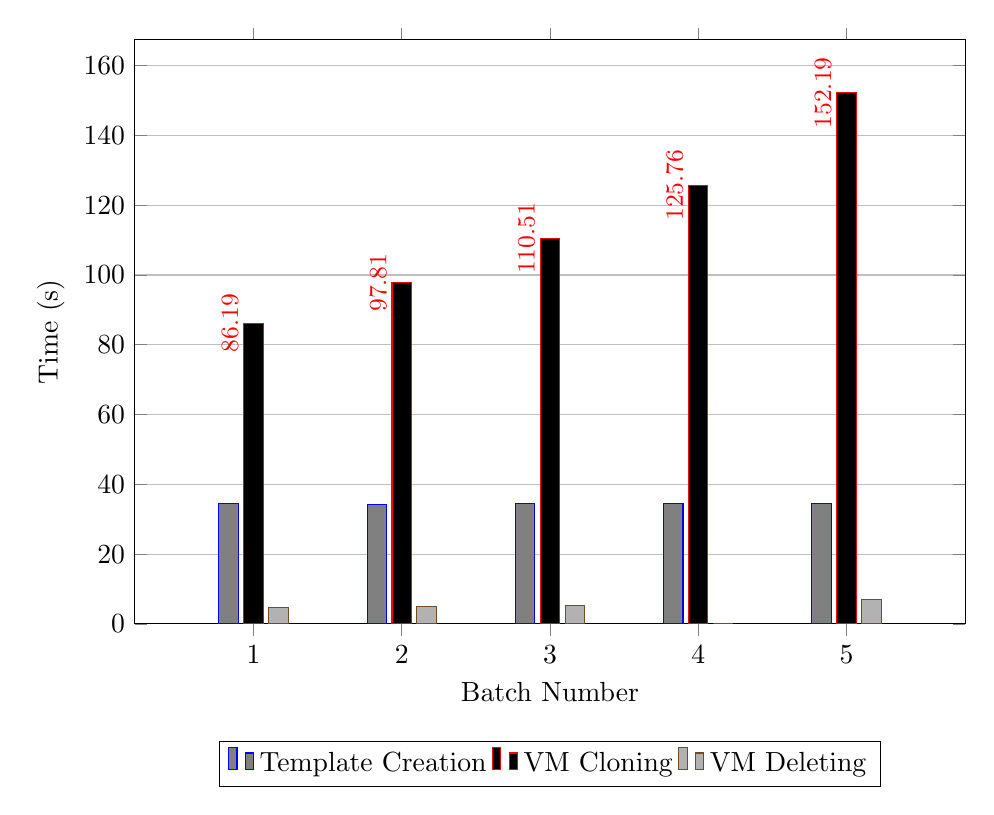
\begin{tikzpicture}
            \begin{axis}[
            ybar,
            bar width=7pt,
            width=\textwidth,
            height=9cm,
            ylabel={Time (s)},
            xlabel={Batch Number},
            symbolic x coords={1,2,3,4,5},
            xtick=data,
            ymin=0,
            enlarge x limits=0.2,
            legend style={at={(0.5,-0.2)}, anchor=north,legend columns=3},
            ymajorgrids=true,
            bar shift auto
            ]

            % Template creation (no labels)
            \addplot+[ybar, fill=gray] coordinates {
            (1,34.379) (2,34.312) (3,34.422) (4,34.609) (5,34.571)
            };
            \addlegendentry{Template Creation}

            % VM cloning (with labels)
            \addplot+[
            ybar,
            fill=black,
            nodes near coords,
            every node near coord/.append style={
                font=\small,
                anchor=south,
                rotate=90,
                yshift=2pt
            }
            ] coordinates {
            (1,86.187) (2,97.805) (3,110.508) (4,125.758) (5,152.186)
            };
            \addlegendentry{VM Cloning}

            % VM deleting (no labels)
            \addplot+[ybar, fill=gray!60] coordinates {
            (1,4.612) (2,4.942) (3,5.377) (4,0.0) (5,7.090)
            };
            \addlegendentry{VM Deleting}

            \end{axis}
        \end{tikzpicture}
        \caption{Grouped bar chart showing VM operation times. Cloning time is labeled to highlight the rising trend. Results
        from Flask running purely sequential code}
        \label{fig:vm_grouped_cloning_focus}
        \end{figure}

        It was also noted that there was an error during the 4th batch of tasks, specifically during the deleting task.

        After some investigation it was found that there were intermittent failures to remove\ac{vm} disks. These failures 
        were \emph{not} detectable via the \ac{pve}\ac{http}\ac{api} responses and only appeared in the\ac{pve} server 
        logs. As orphaned disks accumulated, overall performance degraded significantly.

        \medskip
        \noindent\textbf{Observed Task History Outputs:}
        \begin{verbatim}
--- 1st type of output (VM disks removed successfully) ---
trying to acquire lock...
OK
Logical volume "vm-348786940-disk-0" successfully removed.
TASK OK

--- 2nd type of output (intermittent lock-timeout failures) ---
trying to acquire lock...
Could not remove disk 'local-lvm:vm-120993831-disk-0', check manually:
can't lock file '/var/lock/pve-manager/pve-storage-local-lvm' - got timeout
trying to acquire lock...
OK
Logical volume "vm-120993831-disk-0" successfully removed.
TASK OK

--- 3rd type of output (persistent failures) ---
trying to acquire lock...
Could not remove disk 'local-lvm:vm-363495383-disk-0', check manually:
can't lock file '/var/lock/pve-manager/pve-storage-local-lvm' - got timeout
trying to acquire lock...
can't lock file '/var/lock/pve-manager/pve-storage-local-lvm' - got timeout
TASK OK

--- 4th and final type of output (storage config update errors) ---
trying to acquire lock...
Could not remove disk 'local-lvm:vm-5469324-disk-0', check manually:
can't lock file '/var/lock/pve-manager/pve-storage-local-lvm' - got timeout
trying to acquire lock...
can't lock file '/var/lock/pve-manager/pve-storage-local-lvm' - got timeout
trying to acquire cfs lock 'file-user_cfg' ...
TASK OK
        \end{verbatim}

        This suggests\ac{pve}'s locking mechanism can't keep pace with big amounts of quick sucession delete requests. 
        The lock is used to ensure that two tasks dont modify the\ac{lvm}'s metadata simulatenously. Since there should be 
        some background tasks that are piling up, the system cant keep pace and eventually starts using retries to keep 
        up but even this is insuficient and starts failing more and more towards the end as it becomes fully congested. 
        At the end the system starts becoming overwhelmed and also begins having trouble updating its internal storage 
        config file.  

        This, combined with other factors were the main reason that led us to implement a hard limit on the amount of concurrent 
        requests that can be made from the web application to\ac{pve}\ac{api}. Still, while this significantly reduces the chances 
        of this problem reocurring, it does not fully remedy the problem and additional future work should look into solving this 
        matter completely.

        After performing a cleanup of the orphaned disks we can see that performance was improved from even the 1st baseline test.

        \begin{figure}[h]
        \centering
        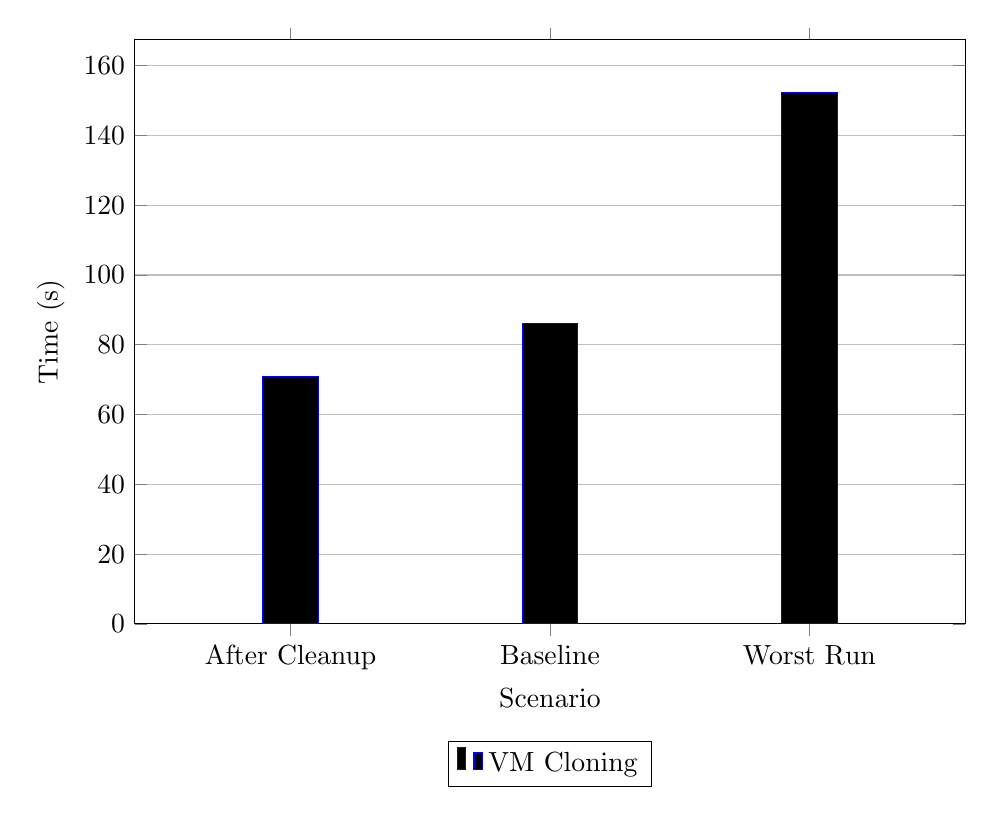
\begin{tikzpicture}
            \begin{axis}[
                ybar,
                bar width=20pt,
                width=\textwidth,
                height=9cm,
                ylabel={Time (s)},
                xlabel={Scenario},
                symbolic x coords={After Cleanup, Baseline, Worst Run},
                xtick=data,
                ymin=0,
                enlarge x limits=0.3,
                legend style={at={(0.5,-0.2)}, anchor=north, legend columns=1},
                ymajorgrids=true
            ]

            % VM cloning bars without labels
            \addplot+[
                ybar,
                fill=black
            ] coordinates {
                (After Cleanup,70.954)
                (Baseline,86.187)
                (Worst Run,152.186)
            };
              
            \addlegendentry{VM Cloning}

            \end{axis}
        \end{tikzpicture}
        \caption{Bar chart showing VM cloning times after cleanup, at baseline, and in the worst case scenario.}
        \label{fig:vm_grouped_cloning_focus}
        \end{figure}




% Write text in here
% Use \subsection and \subsubsection to organize text

